\subsectionaddtolist{سوالات}

\textbf{با انتخاب سوئیچ در CLI و وارد کردن ؟}
\\
اینکار باعث نمایش دستورات و توضیحات آنها می‌شود.
\begin{figure}[h]
    \centering
    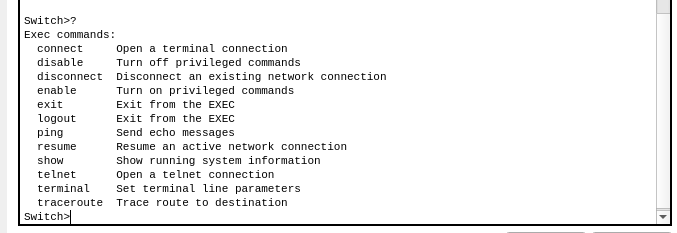
\includegraphics[width=1\textwidth]{img/q/1.png}
\end{figure}

\\
\textbf{عملکرد دستورات}
\\
سوئیچ‌های شبکه، به‌ویژه سوئیچ‌های برند سیسکو، دارای سطوح مختلفی از دسترسی در محیط خط فرمان (CLI) هستند. یکی از این سطوح، \lr{User EXEC Mode} است که پایین‌ترین سطح دسترسی محسوب می‌شود.
\lr{User EXEC Mode} اولین سطحی است که پس از اتصال به سوئیچ از طریق کنسول، Telnet یا SSH وارد آن می‌شوید. این مود فقط اجازه اجرای برخی دستورات نمایشی یا بررسی محدود وضعیت دستگاه را می‌دهد و امکان اعمال تغییرات در پیکربندی سوئیچ را ندارد.برای اعمال تغییر در پیکربندی سوئیچ، نیاز به ورود به حالت \lr{Privileged EXEC} و سپس \lr{Configuration Mode} است.

\begin{itemize}
    \item \lr{enable}: ورود به حالت \lr{Privileged EXEC} برای دسترسی بیشتر
    \item \lr{exit}: خروج از جلسه ترمینال یا بازگشت به مرحله قبلی
    \item \lr{logout}: قطع کامل اتصال از سوئیچ
    \item \lr{ping [آدرس IP]}: ارسال پیام ICMP برای بررسی ارتباط شبکه با مقصد مشخص
    \item \lr{traceroute [آدرس IP]}: ردیابی مسیر بین سوئیچ و یک مقصد مشخص
    \item \lr{show version}: نمایش اطلاعات مربوط به نسخه سیستم‌عامل، سخت‌افزار و uptime دستگاه
    \item \lr{show interfaces}: مشاهده وضعیت فعلی تمام رابط‌های شبکه (interfaces)
    \item \lr{show ip interface brief}: نمایش خلاصه‌ای از وضعیت و پیکربندی IP رابط‌ها
    \item \lr{show mac address-table}: مشاهده جدول نگاشت آدرس‌های MAC شناخته‌شده توسط سوئیچ
    \item \lr{show arp}: نمایش جدول ARP ،نگاشت آدرس‌های IP به MAC
    \item \lr{show history}: مشاهده لیست دستورات وارد شده در نشست جاری
    \item \lr{terminal length}: تعیین تعداد خطوطی که در هر صفحه خروجی CLI نمایش داده می‌شود
    \item \lr{ping ipv6 [آدرس IPv6]}: ارسال پینگ به مقصد دارای آدرس \lr{IPv6}
    \item \lr{traceroute ipv6 [آدرس IPv6]}: ردیابی مسیر ترافیک به مقصد با آدرس \lr{IPv6}
\end{itemize}


\clearpage
\textbf{اجرای دستورات show}
\\
\begin{figure}[h]
    \centering
    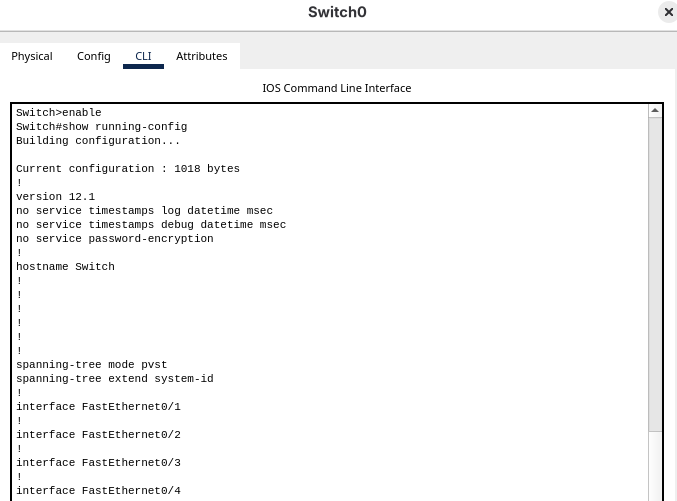
\includegraphics[width=1\textwidth]{img/q/2.png}
\end{figure}
\lr{show running-config}: این دستور تنظیمات روتر و سوئیچ را نمایش می‌دهد.
\\
\begin{figure}[h]
    \centering
    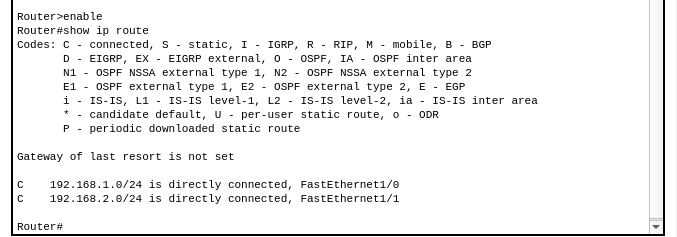
\includegraphics[width=1\textwidth]{img/q/3.png}
\end{figure}
\lr{show ip route}: این دستور فقط برای روتر است و IPهای تنظیم شده بر روی interfaceهای مختلف را نمایش می‌دهد. 
\\
\begin{figure}[h]
    \centering
    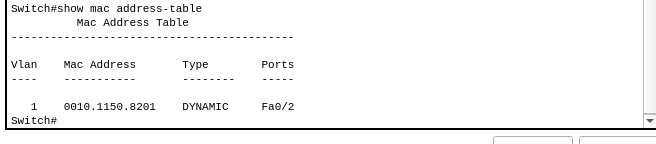
\includegraphics[width=1\textwidth]{img/q/4.png}
\end{figure}
\lr{show mac address-table}: این دستور برای سوئیچ است و آدرس mac دستگاه‌های متصل به سوئیچ را و پورت آن را نمایش می‌دهد. این جدول در هنگام پینگ گرفتن پر می‌شود.
\\
\begin{figure}[h]
    \centering
    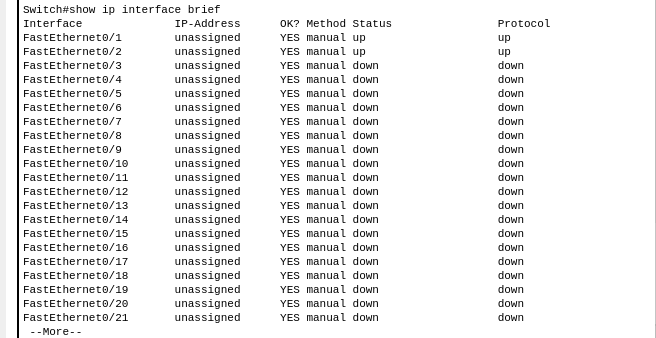
\includegraphics[width=1\textwidth]{img/q/5.png}
\end{figure}
\lr{show ip interface brief}: این دستور \lr{IP address}های مختبف interfaceها را نمایش می‌دهد. و برای سوئیچ و روتر کاربرد دارد.
\\
\begin{figure}[h]
    \centering
    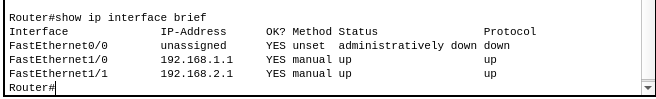
\includegraphics[width=1\textwidth]{img/q/6.png}
\end{figure}
\lr{show vlan brief}: این دستور اطلاعاتی درباره‌ی vlanها می‌دهد و برای سوئیچ قابل اجرا است.
\\
\begin{figure}[h]
    \centering
    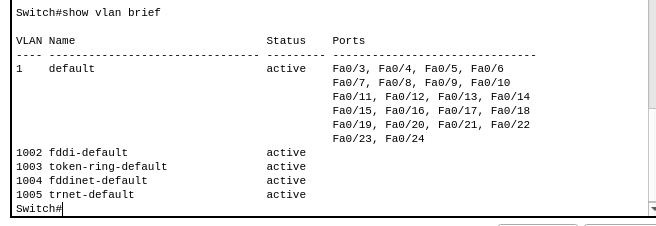
\includegraphics[width=1\textwidth]{img/q/7.png}
\end{figure}

\clearpage
\textbf{gateway}

دروازه پیش‌فرض، دستگاهی در یک شبکه کامپیوتری است که ترافیک شبکه را از یک شبکه به شبکه دیگر هدایت می‌کند. این دستگاه در اکثر شبکه‌ها همان روتر است.
زمانی‌که یک دستگاه (مانند کامپیوتر یا سوئیچ) بخواهد با دستگاهی در خارج از شبکه محلی (LAN) خود ارتباط برقرار کند، بسته‌های اطلاعاتی را به Gateway ارسال می‌کند. Gateway پس از دریافت بسته‌ها، آن‌ها را به مقصد مناسب در شبکه دیگر هدایت می‌کند.
 کاربرد های Gateway :
ایجاد امکان ارتباط بین شبکه‌های محلی مختلف
مسیریابی بسته‌های داده به سمت شبکه‌های دیگر یا اینترنت
کنترل و فیلتر کردن ترافیک ورودی و خروجی
اجرای سیاست‌های امنیتی یا مسیریابی در سطح شبکه

برای مثال اگر کامپیوتری در شبکه‌ای با \lr{IP 192.168.1.10} و \lr{Subnet Mask 255.255.255.0} بخواهد با سروری با \lr{IP 8.8.8.8} ارتباط برقرار کند، ابتدا تشخیص می‌دهد که مقصد در شبکه محلی نیست و بسته را به Gateway، مثلاً \lr{192.168.1.1}، ارسال می‌کند. Gateway این بسته را دریافت کرده و به سمت مقصد هدایت می‌کند.

